\begin{frame}{Reinforcement learning}
	
	\begin{center}
		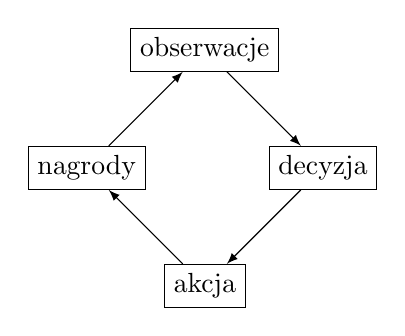
\begin{tikzpicture}
			\node[draw] at (0, 1.5) (1) {obserwacje};
			\node[draw] at (1.5, 0) (2) {decyzja};
			\node[draw] at (0, -1.5) (3) {akcja};
			\node[draw] at (-1.5, 0) (4) {nagrody};
			\draw [->,-latex] (1) to (2);
			\draw [->,-latex] (2) to (3);
			\draw [->,-latex] (3) to (4);
			\draw [->,-latex] (4) to (1);
		\end{tikzpicture}
	\end{center}
	
\end{frame}
